Nodes will double $CW(k)$ after collisions and reset it ($CW(k)=CW_{min}$) upon each transmission success, augmenting the collision probability. Because CSMA/ECA is totally distributed, the number of nodes ($N$) is unknown to all contenders. Therefore, $CW(k)$ is used to relate collisions to the number of users in the system.

%$N$ is unknown to all contenders, so $CW(k)$ is the only indicator for each node of the current state of the system.

To make it possible to achieve a collision-free state when the system is overcrowded ($N>N_{\max}$), we instruct nodes not to reset $CW(k)$ after successful transmissions and modify the collision-free constraint to~$N_{\max}=CW(k)/2$. This is called \emph{hysteresis} from here forward.

Hysteresis forces nodes to \emph{stick} to the value of the current backoff stage, $k$; resulting in a larger $CW(k)$. This measure leads to a collision-free state while $N\leq N_{\max}$.

Having a greater collision-free constraint means that more nodes are able to achieve a collision-free state. Nevertheless, in a $N\leq N_{\max}$ scenario, contenders may have different deterministic backoff counters which provoke some nodes to access the channel more often than others. This fairness issue is averted with \emph{fair-share}.

Fair-share consist in allowing each contender to send $2^{k}$ packets at every transmission, making sure that contenders with longer backoff are compensated proportionally.

Figure~\ref{fig:fairShare}, depicts how CSMA/ECA with hysteresis and fair-share achieves greater throughput than CSMA/ECA alone, maintaining a collision-free state while being fair (Jain's Fairness Index~\cite{JFI}~(JFI) equal to $1$), for any number of contenders.

\begin{figure}[htbp]
  \centering
  \includegraphics[width=0.7\linewidth, angle = -90]{figures/errorPlots/ECA-w-enhancements-fixed.eps}
  \caption{Throughput and Jain's Fairness Index when implementing fair-share in CSMA/ECA
  \label{fig:fairShare}}
\end{figure}

The concept of fair-share, was first introduced by Fang et al. in~\cite{L_MAC2}. This work evaluates the performance of CSMA/ECA when implementing the concept in a customized C++ simulator.

\section{Evaluation}
CSMA/ECA preserves backward compatibility with CSMA/CA (details in~\cite{CSMA_ECA}~and~\cite{HE}), which is paramount for the coexistence and progressive adoption of the protocol. 

%Other performance evaluations, like a semi-analytical framework modelling the enhanced collision avoidance mechanism and comparing it with other access schemes (like Basic Access and RTS/CTS), are provided in~\cite{E2CA_performance}. Nevertheless, to the best of our knowledge this is the first evaluation of resilience and fair-share in CSMA/ECA.

Implementation is performed on a customized version of the COST~\cite{COST}~simulator. The system was set to be under saturation (nodes always have packets to transmit) during a period of ten seconds at a maximum throughput of $11$Mbps. The number of contenders ranges from $2$ to $50$ and a hundred simulations are performed for each number of contenders. Further MAC-related parameters can be found under~\emph{stats/stats.h}~in~\cite{sim:parameters}; as well as the code for the whole CSMA/ECA implementation.

Figure~\ref{fig:throughput} and Figure~\ref{fig:fairShare} are results derived from the evaluation platform with $95\%$ confidence intervals.